\documentclass[a4paper, 11pt]{article}

%% Language and font encodings
\usepackage[english]{babel}
\usepackage[utf8x]{inputenc}
\usepackage[T1]{fontenc}
\usepackage{float}

%% Sets page size and margins
\usepackage[a4paper,top=3cm,bottom=2cm,left=3cm,right=3cm,marginparwidth=1.75cm]{geometry}

%% Useful packages
\usepackage{amsmath}
\usepackage{graphicx}
\usepackage[colorinlistoftodos]{todonotes}
\usepackage[colorlinks=true, allcolors=blue]{hyperref}

\renewcommand{\figurename}{Figura}

\title{Rede Neuronal com Backpropagation}
\author{João Francisco B. S. Martins}
\date{16 de Maio de 2017}

\begin{document}
\maketitle
\section{Introdução}
Redes neuronais são modelos computacionais inspirados na forma como a redes neuronais nos cérebros dos seres vivos processam informações. Elas são compostas por camadas, que por sua vez são compostas por unidades, as quais chamamos de neurônios por mimificarem o comportamento de suas contrapartes reais. Cada neurônios em uma camada se liga a todos da camada seguinte e essas ligações possuem pesos, os quais são atualizados, através da técnica de backpropagation, a cada rodada processamento de informações(forward propagation) realizada pela rede. Apesar do algoritmo de backpropagation ter sido publicado inicialmente na década de 70, somente nos últimos anos o aprendizado de máquina com redes neuronais se tornou uma tecnologia utilizada em escala global, também se tornando uma das maiores áreas de pesquisa em computação, muito disso devido a invenção da técnica de aprendizado profundo(Deep Learning). 

Nesse trabalho implementaremos uma rede neuronal de 3 camadas a qual utiliza o algoritmo de backpropagation para atualizar seus pesos. A base de dados utilizada foi a MNIST handwritten digit database.

\section{Modelagem e Implementação}
A base MNIST conta com 784 atributos de entrada, onde cada um corresponde a um pixel numa imagem 28 x 28, e 1 atributo de saída que representa o número escrito naquela imagem. Já nossa rede terá 784 neurônios de entrada + 1 neurônio de bias na camada de entrada, 10 neurônios na camada de saída, pois nossa rede utiliza one hot encoding(um neurônio por classe de saída), e número variável de neurônios na camada escondida. Essa variação não ocorrerá apenas no tamanho da camada escondida, mas também na taxa de aprendizado e no tamanho do batch da descida de gradiente, para que possamos fazer comparações e discutir os resultados.

Para implementarmos a rede em si fizemos um código orientado a objetos em Python. O código está distribuído em dois arquivos: \textit{neural\_network.py} e \textit{main.py}. O primeiro contém a declaração e implementação da classe \textbf{NeuralNetwork}, a qual descreve a rede neural como duas matrizes de pesos e executa as operações de forward e backpropagation. O segundo módulo contém o código principal, que com apenas algumas linhas cria e treina a rede de acordo com os argumentos variáveis passados em sua chamada. O uso da biblioteca \textbf{numpy} para manipulação de arrays e realização de operações de álgebra linear foi essencial, não apenas por fornecer uma estrutura de dados concisa mas também por agilizar as operações em muitas ordens de grandeza.

\subsection{Execução}
O código pode ser executado através da seguinte chamada:
\begin{equation*}
\text{python \textbf{main.py} \textit{<output\_file> <n\_hidden> <batch\_size> <l\_rate>}}
\end{equation*}

\begin{itemize}
  \item \textit{<output\_file>}: Caminho para os arquivos de saída onde o erro empírico por época deve ser salvo.
  \item \textit{<n\_hidden>}: Número de unidades na camada escondida excluindo a unidade de bias.
  \item \textit{<batch\_size>}: Tamanho do batch usado na descida de gradiente:
  	\begin{itemize}
        \item \textbf{Stochastic Gradient Descent}: batch\_size = 1.
        \item \textbf{Mini-batch Gradient Descent}: 1 < batch\_size < número de instâncias de entrada.
        \item \textbf{Batch Gradient Descent}: batch\_size = número de instâncias de entrada.
    \end{itemize}
  \item \textit{<l\_rate>}: Taxa de aprendizado da rede utilizada na atualização dos pesos.
\end{itemize}
 
Também é possível executar o script diretamente com os comandos: \par
\textbf{>} chmod +x ./main \par
\textbf{>} ./main <ARGS>
				


\subsection{Criação da Rede}
Inicialmente carregamos toda a base de dados num array de arrays do numpy, convertendo a saída esperada para o formato de one hot encoding e separando os atributos de entrada e saída. Os atributos de entrada são normalizados para que todos estejam entre 0 e 1, impedindo inconsistências no treinamento da rede. Assim poupamos tempo computacional, não tendo que acessar o arquivo de dados a cada iteração.

Assim que temos nossa base de dados estruturada, criamos a rede neural passando o número fixo de neurônios de entrada(784) e neurônios de saída(10) assim como um número variável de neurônios escondidos, recebido por argumento na chamada do programa. Os pesos são inicializados aleatoriamente com valores entre $-0.001$ e $0.001$. Assim que a rede for inicializada chamamos a função \textbf{train}, que cuidará do processo de treino da rede no dataset com os parâmetros fornecidos. Essas são as únicas duas chamadas necessárias no módulo principal.

\subsection{Treino}
A função de treino, \textbf{train()} recebe os parâmetros \textbf{x}, \textbf{y}, \textbf{n\_epoch}, \textbf{batch\_size}, \textbf{l\_rate} e \textbf{output\_file}. A maioria desses parâmetros foi passado na execução do programa, com exceção de \textbf{x}, que são os inputs do dataset, \textbf{y}, que são os outputs em one hot encoding e \textbf{n\_epoch} que corresponde ao número de épocas a serem executadas(fixado em 100). A mesma função executa todos os algoritmos de descida de gradiente variando apenas o batch\_size, como já explicado na subseção 2.1. O algoritmo calcula então o número de batches que serão executados em uma época, ao definir o tamanho de cada época como o número de instâncias na base de dados(5000), e inicia um loop. A cada instância dentro de um batch, realizamos o forward propagation das entradas da instância e calculamos os deltas para os sinais de ativação gerados. Somente ao fim de um batch  é que atualizamos os pesos com os deltas calculados.
\subsubsection{Forward Propagation}
Para propagarmos os erros primeiramente fazemos com que as ativações da camada de entrada sejam iguais aos atributos de entrada para a instância corrente, os quais já apresentam o valor de ativação 1 para o neurônio de bias. Para calcularmos os valores de ativação da camada escondida propagamos os valores da primeira camada ao multiplicarmo-os pelos respectivos pesos de suas conexões e usarmos a função de ativação, que no caso é a sigmoide, para sabermos se o neurônio passará aquele valor a diante ou não. A função sigmoide é dada por:

\begin{equation*}
\sigma(x) = \frac{1}{1 + e^{-x}}
\end{equation*}

Ao calcularmos a ativação de um neurônio considerando todas as suas entradas multiplicadas pelos pesos, temos o valor que aquele componente passará para frente, ao repetirmos o mesmo procedimento para camada seguinte. Por fim teremos a ativação dos neurônios na camada de saída, a qual corresponderá, obviamente, à saída da rede.

\subsubsection{Cálculo dos Deltas}
O cálculo dos deltas é a primeira parte(de duas) do algoritmo de backpropagation. Cada neurônio das duas últimas camadas possuí um delta próprio, com exceção do neurônio de bias da camada escondida. Para calcularmos o delta de um neurônio da camada de saída, subtraímos o valor da ativação da mesma pelo valor esperado para aquela instância e logo em seguida multiplicamos esse resultado pelo valor da derivada da sigmoide da ativação daquele neurônio. A derivada da sigmoide é dada pela regra da cadeia:

\begin{equation*}
\sigma'(x) = \sigma(x) \dot (1 - \sigma(x))
\end{equation*}

Para calcularmos o delta das unidades da camada escondida(exceto para o bias), multiplicamos os pesos das conexões entre as duas camadas pelo delta do respectivo neurônio na camada de saída, para, logo em sequência, multiplicarmos o resultado pela derivada da sigmoide da ativação do respectivo neurônio na camada escondida

Como disponibilizamos algoritmos de descida de gradiente em batch, precisamos acumular os deltas até o fim de um batch, quando então atualizaremos os pesos. Como também precisamos guardar os valores de ativação da rede para aquela instância, fazemos o produto dos dois e salvamos em uma variável \textbf{DELTA}.

\subsubsection{Atualização dos Pesos}
A atualização dos pesos é o segundo e último passo do backpropagation. Ao fim de um batch, temos o somatório do produto dos deltas pela ativação, a cada instância, armazenado em DELTA. Para atualizarmos os pesos simplesmente utilizamos a regra delta:

\begin{equation*}
w_{i+1} = w_{i} - r * \Delta
\end{equation*}

Onde $r$ é a taxa de aprendizado da rede e $\Delta$ é o acumulador DELTA. A fórmula é a mesma para os pesos de todas as camadas.

\subsubsection{Erro Empírico}
O erro empírico é calculado ao fim de cada batch, e quando no fim de uma época, associamos o erro naquela época ao erro do último batch executado na mesma. O erro é dado pela função de custo de entropia cruzada(Cross-entropy cost function) a seguir:
\begin{equation*}
C = -\frac{1}{n}\sum_{x}\sum_{j}[ y_j \ln a^{L}_{j} + (1 - y_j) \ln (1 - a^{L}_{j})].
\end{equation*}

\subsubsection{Resultados do Treino}

Os resultados do treino foram salvos num arquivo de extensão \textbf{csv} de nome igual à string \textbf{output\_file}, recebida na chamada da função de treino. Esse arquivo tem 2 colunas e número de linhas correspondente a quantidade de épocas pois ao fim de cada época salvamos o índice da mesma e o erro empírico encontrado, nessa ordem. 

\section{Análise dos Experimentos}

Ao todo foram pedidos 36 testes diferentes, criados ao variarmos os atributos \textbf{número de unidades escondidas}, \textbf{tamanho do batch}(algoritmo de gradiente) e \textbf{taxa de aprendizado}. Os gráficos abaixo foram plotados usando os dados salvos após cada teste como explicado na subseção 2.3.5, e foram agrupados por taxa de aprendizado para facilitar a visualização dos resultados e comparação entre eles.

\subsection{Taxa de aprendizado igual a 0.5}

\begin{figure}[h]	
\centering
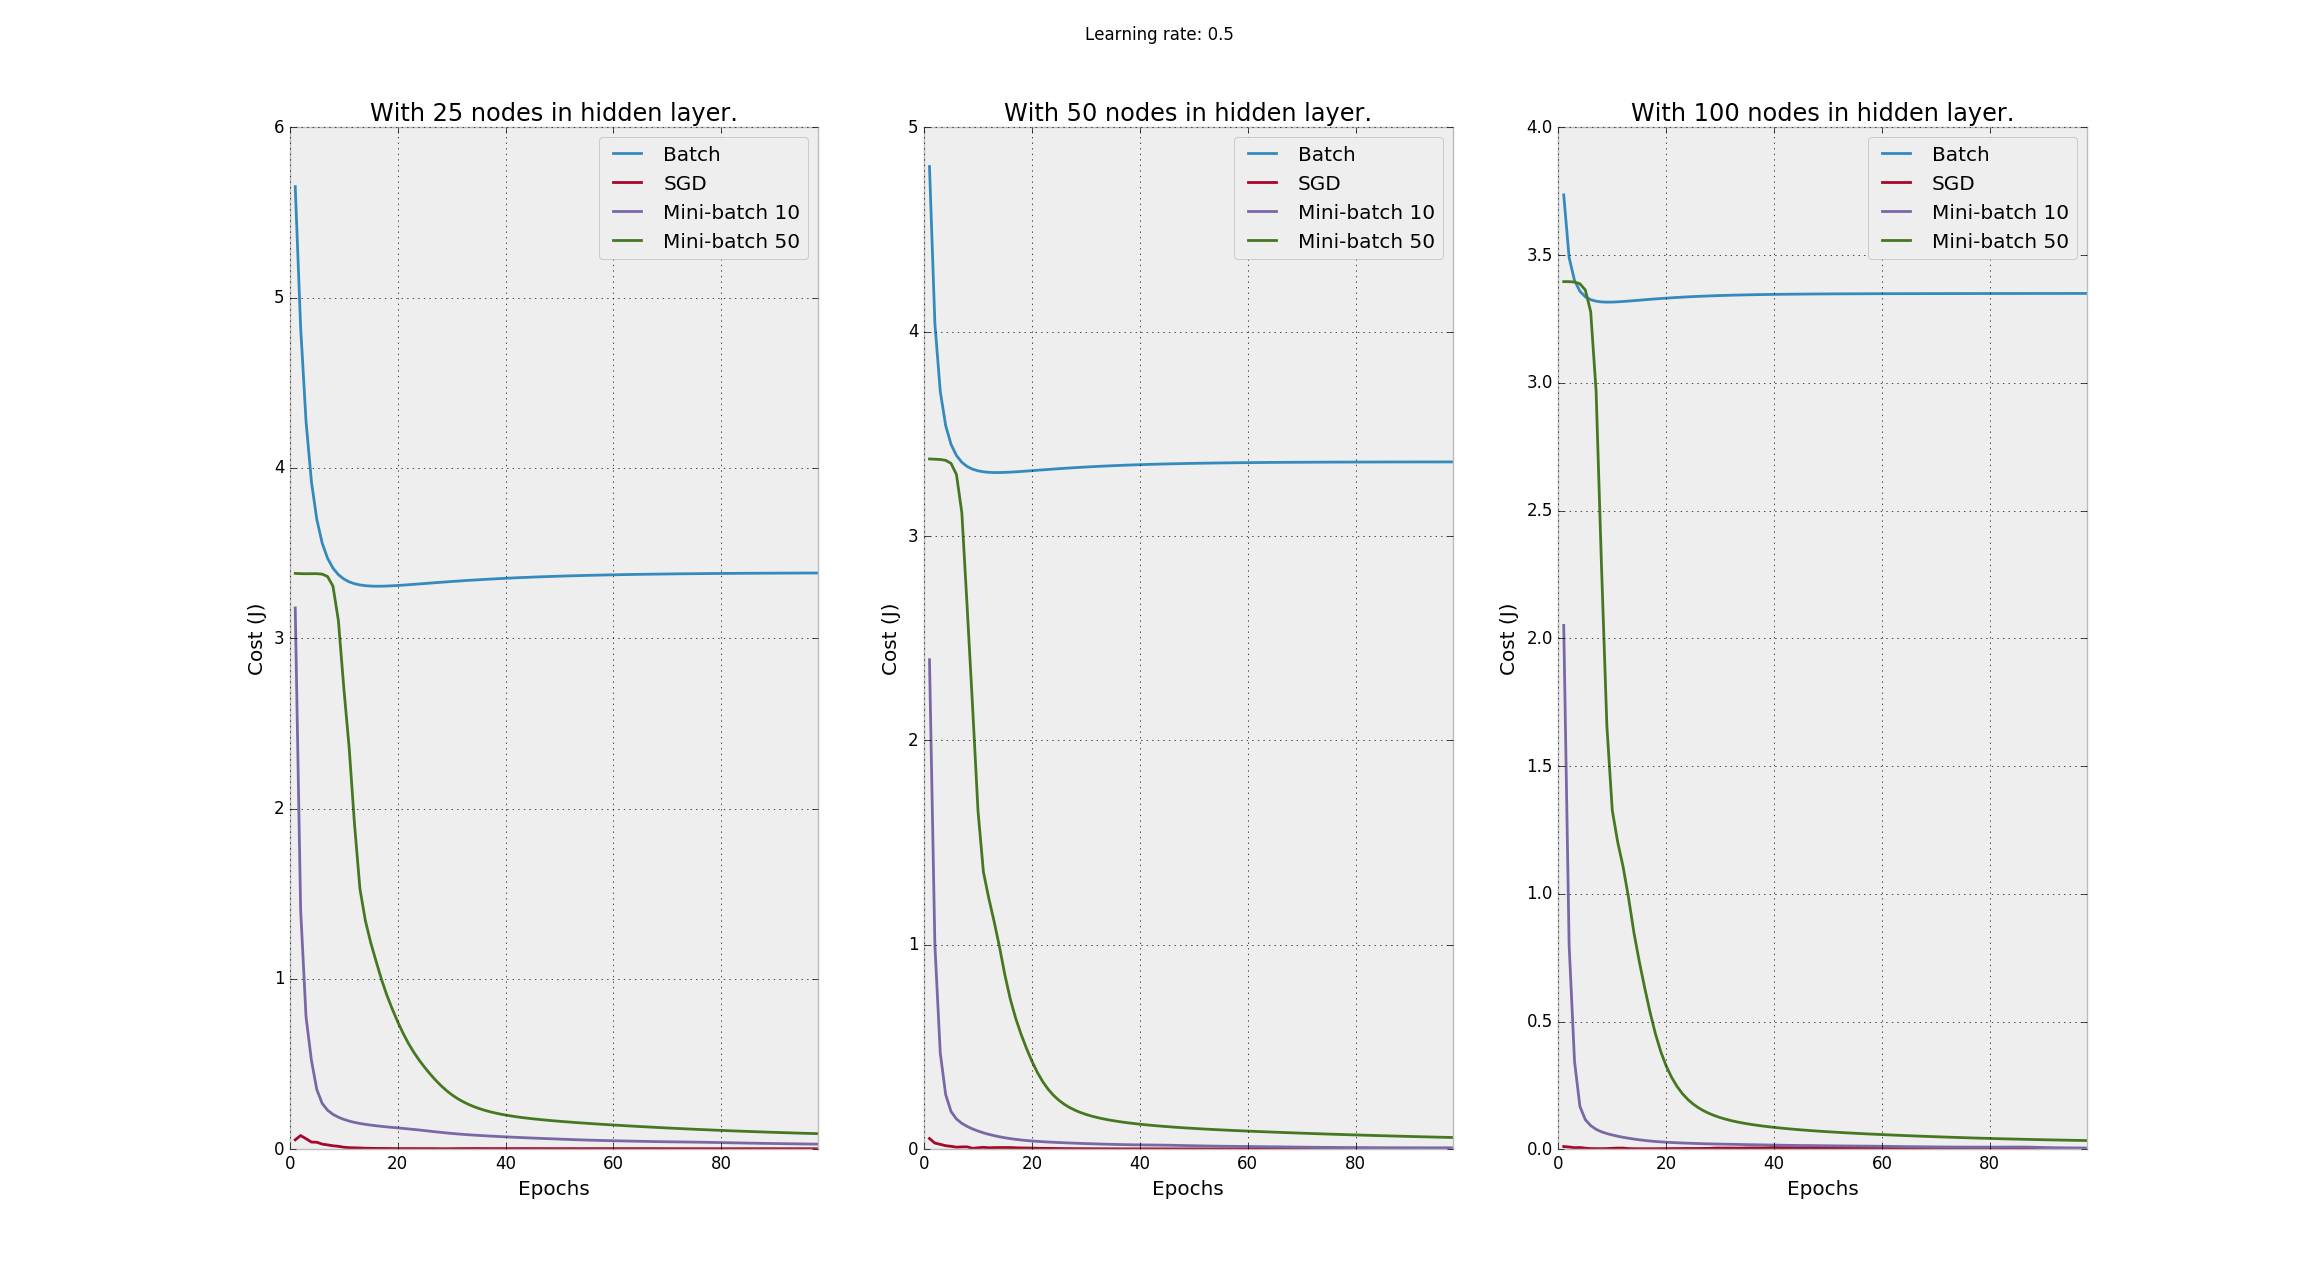
\includegraphics[width=\textwidth,height=\textheight,keepaspectratio]{5.png}
\caption{Erro empírico/época para taxa de aprendizado igual 0.5}
\end{figure}

Podemos ver que a rede converge lentamente, levando entre 60 e 80 épocas para chegar em um valor razoável de erro, em todos os três gráficos. Olhando para o número de unidades na camada escondida é fácil notar que, quanto mais unidades, mais rápido a rede converge, uma vez que temos uma capacidade de ajuste fino maior. 

O algoritmo SGD é o que converge mais rápido e mais minimiza o erro, porque atualiza os pesos muito mais vezes que os outros, seguido do mini-batch 10 e do mini-batch 50, ou seja, quanto mais atualizamos os pesos mais rápido convergimos e melhor é o nosso erro .Infelizmente, como não implementamos momentum, o algoritmo de batch caiu em um mínimo local, e mesmo tentando sair dessa região, como podemos perceber pelo leve aumento do erro, ele foi incapaz de o fazer, mantendo o erro bem alto em comparação com os outros.

\subsection{Taxa de aprendizado igual a 1}

\begin{figure}[h]	
\centering
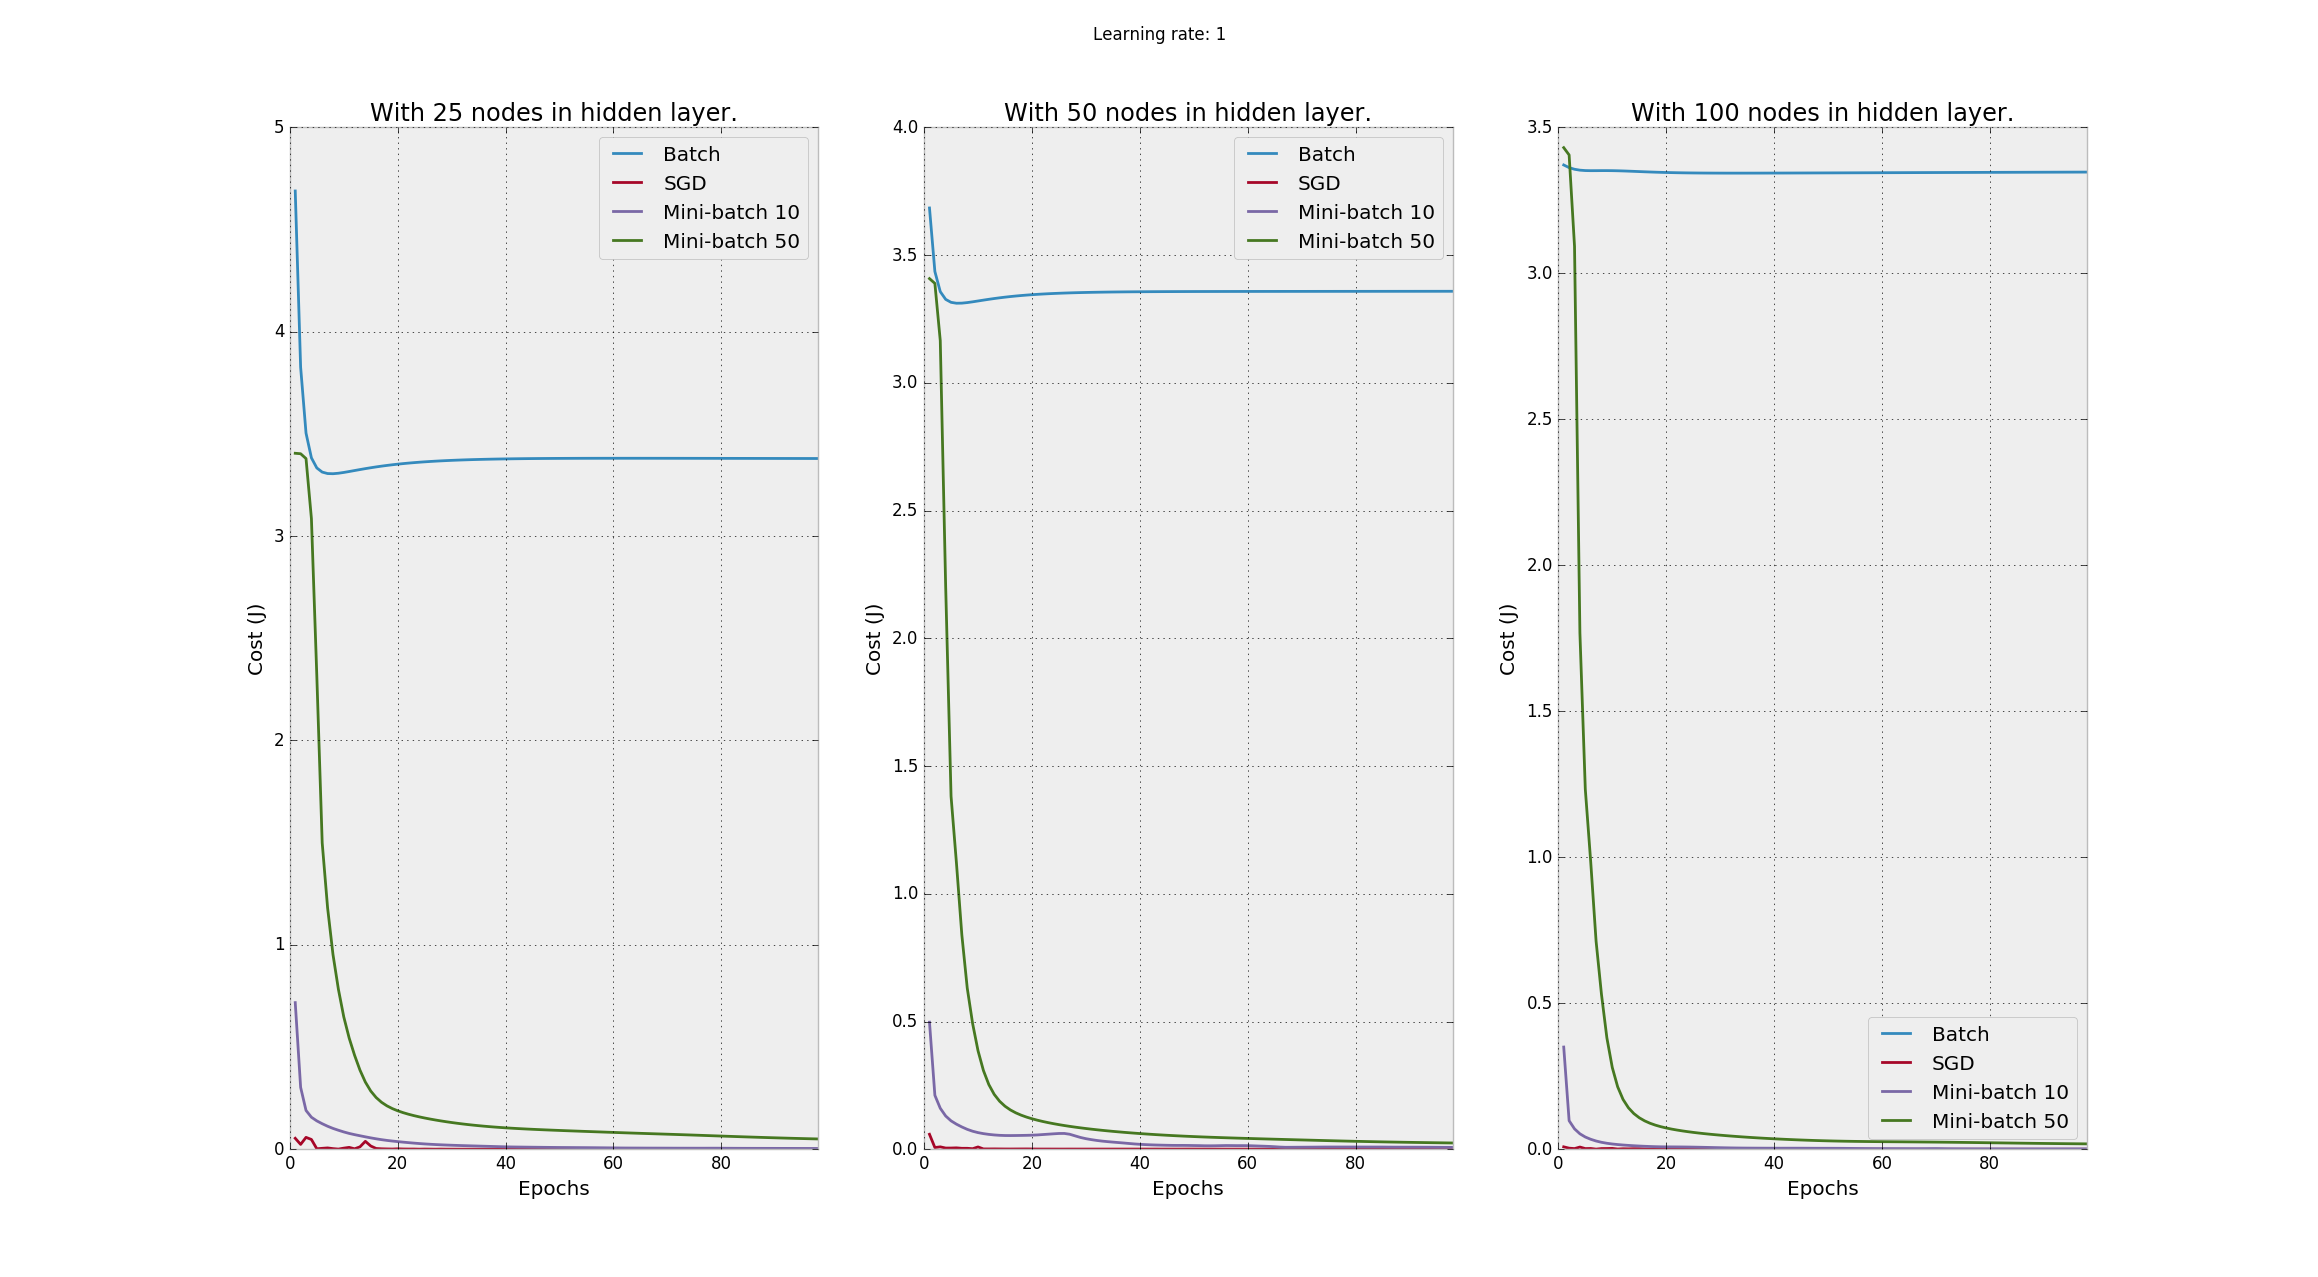
\includegraphics[width=\textwidth,height=\textheight,keepaspectratio]{1.png}
\caption{Erro empírico/época para taxa de aprendizado igual 1}
\end{figure}

O padrão aqui se repete, porém o erro converge mais rápido, devido a uma taxa de aprendizado maior. A ordem dos algoritmos ainda é a mesma que no gráfico anterior, o número de unidades escondidas ainda faz com que o erro tenha uma convergência mais rápida e novamente a descida de gradiente em batch caiu no mínimo local.



\subsection{Taxa de aprendizado igual a 10}

\begin{figure}[!htb]	
\centering
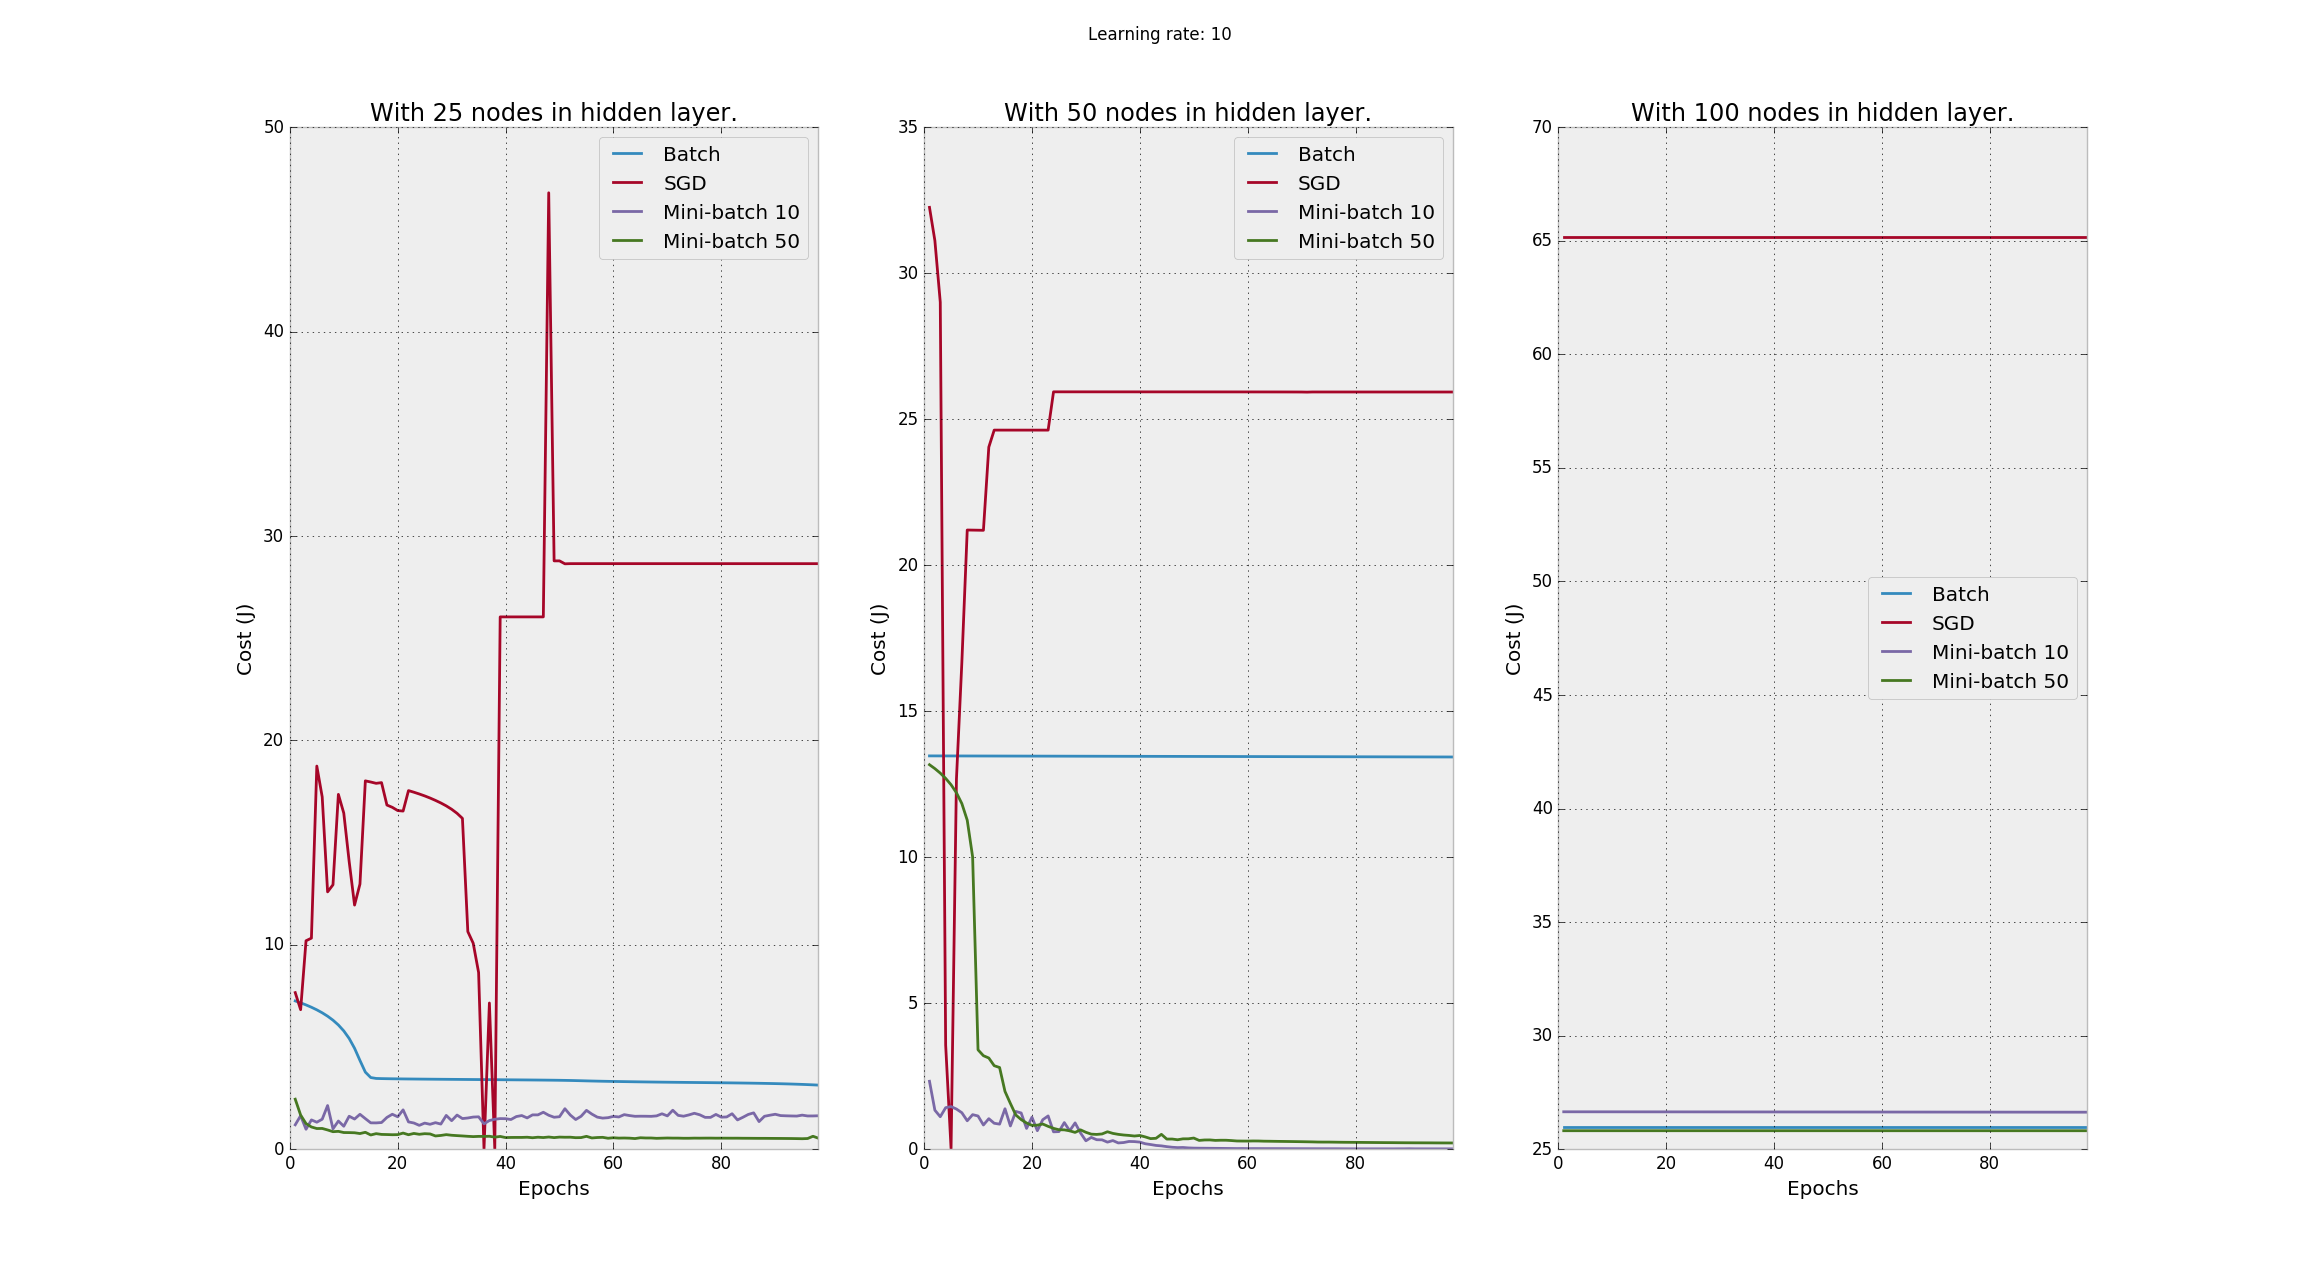
\includegraphics[width=\textwidth,height=\textheight,keepaspectratio]{10.png}
\caption{Erro empírico/época para taxa de aprendizado igual 10}
\end{figure}

Aqui o cenário muda completamente. Com uma taxa de aprendizado tão grande, os resultados ficam caóticos e imprevisíveis na maioria dos casos, custando a convergir para os números mais baixos de neurônios escondidos. É interessante ver que com 100 neurônios na camada escondida os erros convergem, mesmo que o valor do erro seja muito grande, como é o caso da descida de gradiente estocástico, que nesses experimentos ficou em últimos em todos os gráficos(diferindo dos resultados prévios). Isso ocorreu pelo mesmo de antes: ela atualiza os pesos muito mais vezes do que seus concorrentes, fazendo com que a divergência seja muito mais provável.

O plot para taxa de aprendizado 10 se encontra na próxima página.



\section{Conclusão}

Esse foi um dos trabalhos práticos mais divertidos e ao mesmo tempo desafiadores que eu já implementei. Foi muito interessante ver a rede convergindo e saber que aquela era uma criação minha. É difícil compreender aqueles que, quando se referindo a aprendizagem de máquina, dizem "É o homem querendo brincar de Deus!", quando se vê algo tão bonito evoluindo diante dos seus olhos.

Além de me familiarizar ainda mais com os conceitos de redes neurais de várias camadas, a medida que eu ia programando, minha expertise com a biblioteca \textit{numpy} aumentou consideravelmente, assim como meus conhecimentos de plots de gráficos usando as bibliotecas \textit{matplotlib} e \textit{pandas}. Por fim, este TP foi extremamente proveitoso.

\end{document}